\documentclass[twoside]{book}

% Packages required by doxygen
\usepackage{fixltx2e}
\usepackage{calc}
\usepackage{doxygen}
\usepackage{graphicx}
\usepackage[utf8]{inputenc}
\usepackage{makeidx}
\usepackage{multicol}
\usepackage{multirow}
\PassOptionsToPackage{warn}{textcomp}
\usepackage{textcomp}
\usepackage[nointegrals]{wasysym}
\usepackage[table]{xcolor}

% Font selection
\usepackage[T1]{fontenc}
\usepackage{mathptmx}
\usepackage[scaled=.90]{helvet}
\usepackage{courier}
\usepackage{amssymb}
\usepackage{sectsty}
\renewcommand{\familydefault}{\sfdefault}
\allsectionsfont{%
  \fontseries{bc}\selectfont%
  \color{darkgray}%
}
\renewcommand{\DoxyLabelFont}{%
  \fontseries{bc}\selectfont%
  \color{darkgray}%
}
\newcommand{\+}{\discretionary{\mbox{\scriptsize$\hookleftarrow$}}{}{}}

% Page & text layout
\usepackage{geometry}
\geometry{%
  a4paper,%
  top=2.5cm,%
  bottom=2.5cm,%
  left=2.5cm,%
  right=2.5cm%
}
\tolerance=750
\hfuzz=15pt
\hbadness=750
\setlength{\emergencystretch}{15pt}
\setlength{\parindent}{0cm}
\setlength{\parskip}{0.2cm}
\makeatletter
\renewcommand{\paragraph}{%
  \@startsection{paragraph}{4}{0ex}{-1.0ex}{1.0ex}{%
    \normalfont\normalsize\bfseries\SS@parafont%
  }%
}
\renewcommand{\subparagraph}{%
  \@startsection{subparagraph}{5}{0ex}{-1.0ex}{1.0ex}{%
    \normalfont\normalsize\bfseries\SS@subparafont%
  }%
}
\makeatother

% Headers & footers
\usepackage{fancyhdr}
\pagestyle{fancyplain}
\fancyhead[LE]{\fancyplain{}{\bfseries\thepage}}
\fancyhead[CE]{\fancyplain{}{}}
\fancyhead[RE]{\fancyplain{}{\bfseries\leftmark}}
\fancyhead[LO]{\fancyplain{}{\bfseries\rightmark}}
\fancyhead[CO]{\fancyplain{}{}}
\fancyhead[RO]{\fancyplain{}{\bfseries\thepage}}
\fancyfoot[LE]{\fancyplain{}{}}
\fancyfoot[CE]{\fancyplain{}{}}
\fancyfoot[RE]{\fancyplain{}{\bfseries\scriptsize Generated on Thu Jul 27 2017 15\+:06\+:16 for S\+N56\+H\+C164 by Doxygen }}
\fancyfoot[LO]{\fancyplain{}{\bfseries\scriptsize Generated on Thu Jul 27 2017 15\+:06\+:16 for S\+N56\+H\+C164 by Doxygen }}
\fancyfoot[CO]{\fancyplain{}{}}
\fancyfoot[RO]{\fancyplain{}{}}
\renewcommand{\footrulewidth}{0.4pt}
\renewcommand{\chaptermark}[1]{%
  \markboth{#1}{}%
}
\renewcommand{\sectionmark}[1]{%
  \markright{\thesection\ #1}%
}

% Indices & bibliography
\usepackage{natbib}
\usepackage[titles]{tocloft}
\setcounter{tocdepth}{3}
\setcounter{secnumdepth}{5}
\makeindex

% Hyperlinks (required, but should be loaded last)
\usepackage{ifpdf}
\ifpdf
  \usepackage[pdftex,pagebackref=true]{hyperref}
\else
  \usepackage[ps2pdf,pagebackref=true]{hyperref}
\fi
\hypersetup{%
  colorlinks=true,%
  linkcolor=blue,%
  citecolor=blue,%
  unicode%
}

% Custom commands
\newcommand{\clearemptydoublepage}{%
  \newpage{\pagestyle{empty}\cleardoublepage}%
}


%===== C O N T E N T S =====

\begin{document}

% Titlepage & ToC
\hypersetup{pageanchor=false,
             bookmarks=true,
             bookmarksnumbered=true,
             pdfencoding=unicode
            }
\pagenumbering{roman}
\begin{titlepage}
\vspace*{7cm}
\begin{center}%
{\Large S\+N56\+H\+C164 }\\
\vspace*{1cm}
{\large Generated by Doxygen 1.8.8}\\
\vspace*{0.5cm}
{\small Thu Jul 27 2017 15:06:16}\\
\end{center}
\end{titlepage}
\clearemptydoublepage
\tableofcontents
\clearemptydoublepage
\pagenumbering{arabic}
\hypersetup{pageanchor=true}

%--- Begin generated contents ---
\chapter{S\+N54\+H\+C164.\+h Routines for usage of S\+N54\+H\+C164 8-\/bit shift register.}
\label{index}\hypertarget{index}{}This file provides functions for usage of serial 8-\/bit shift register S\+N54\+H\+C164. In addition a sample (\hyperlink{main_8c}{main.\+c}) is included to show how to use it. This sample is based on an A\+Tmega328\+P micro controller.

Datasheets can be found here\+:

\href{../datasheets/Atmel-42735-8-bit-AVR-Microcontroller-ATmega328-328P_Datasheet.pdf}{\tt A\+Tmega328\+P} ~\newline
 \href{../datasheets/164445-da-01-en-CMOS_IC_SN74HC164N_DIP14_TID.pdf}{\tt S\+N54\+H\+C164} 
\chapter{File Index}
\section{File List}
Here is a list of all files with brief descriptions\+:\begin{DoxyCompactList}
\item\contentsline{section}{/home/woifal/\+Projekte/avr/\+S\+N54\+H\+C164/code/\hyperlink{main_8c}{main.\+c} \\*Usage demonstration of Shift Register S\+N54\+H\+C164 (\hyperlink{_s_n54_h_c164_8h}{S\+N54\+H\+C164.\+h}) }{\pageref{main_8c}}{}
\item\contentsline{section}{/home/woifal/\+Projekte/avr/\+S\+N54\+H\+C164/code/\hyperlink{_s_n54_h_c164_8c}{S\+N54\+H\+C164.\+c} \\*Functions for Shift Register S\+N54\+H\+C164 }{\pageref{_s_n54_h_c164_8c}}{}
\item\contentsline{section}{/home/woifal/\+Projekte/avr/\+S\+N54\+H\+C164/code/\hyperlink{_s_n54_h_c164_8h}{S\+N54\+H\+C164.\+h} \\*Functions for Shift Register S\+N54\+H\+C164 }{\pageref{_s_n54_h_c164_8h}}{}
\end{DoxyCompactList}

\chapter{File Documentation}
\hypertarget{main_8c}{\section{/home/woifal/\+Projekte/avr/\+S\+N54\+H\+C164/code/main.c File Reference}
\label{main_8c}\index{/home/woifal/\+Projekte/avr/\+S\+N54\+H\+C164/code/main.\+c@{/home/woifal/\+Projekte/avr/\+S\+N54\+H\+C164/code/main.\+c}}
}


Usage demonstration of Shift Register S\+N54\+H\+C164 (\hyperlink{_s_n54_h_c164_8h}{S\+N54\+H\+C164.\+h})  


{\ttfamily \#include $<$avr/io.\+h$>$}\\*
{\ttfamily \#include \char`\"{}S\+N54\+H\+C164.\+h\char`\"{}}\\*
Include dependency graph for main.\+c\+:\nopagebreak
\begin{figure}[H]
\begin{center}
\leavevmode
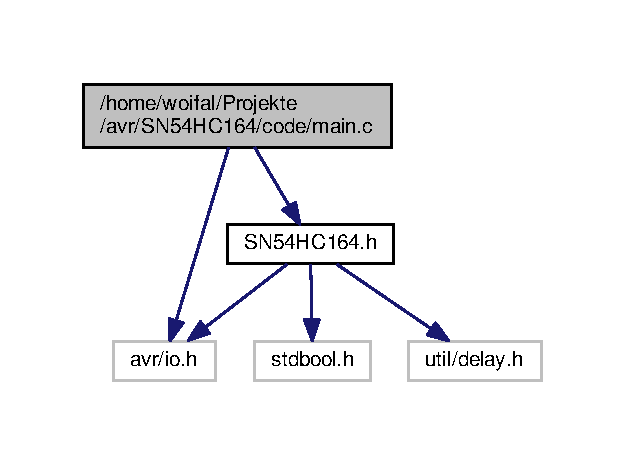
\includegraphics[width=300pt]{main_8c__incl}
\end{center}
\end{figure}
\subsection*{Macros}
\begin{DoxyCompactItemize}
\item 
\#define \hyperlink{main_8c_a72559d8c18a43489198ac2c8a34097bb}{S\+H\+I\+F\+T\+\_\+\+R\+E\+G\+\_\+\+D\+A\+T\+A\+\_\+\+P\+I\+N}~P\+D2
\item 
\#define \hyperlink{main_8c_a15681ea050f8feb5f46ef1bf67341845}{S\+H\+I\+F\+T\+\_\+\+R\+E\+G\+\_\+\+C\+L\+R\+\_\+\+P\+I\+N}~P\+D3
\item 
\#define \hyperlink{main_8c_a5183e6a3912ceb97eaf2801b1950a5c5}{S\+H\+I\+F\+T\+\_\+\+R\+E\+G\+\_\+\+C\+L\+K\+\_\+\+P\+I\+N}~P\+D4
\item 
\#define \hyperlink{main_8c_aded34a8ca3d810dae7b267f7ba2fd116}{S\+H\+I\+F\+T\+\_\+\+R\+E\+G\+\_\+\+D\+A\+T\+A\+\_\+\+P\+O\+R\+T}~P\+O\+R\+T\+D
\item 
\#define \hyperlink{main_8c_a51bf538decb2026cc3bd721b62c1aee8}{S\+H\+I\+F\+T\+\_\+\+R\+E\+G\+\_\+\+D\+A\+T\+A\+\_\+\+D\+I\+R\+\_\+\+R\+E\+G}~D\+D\+R\+D
\item 
\#define \hyperlink{main_8c_a6793f41a796654c703c7f7bfa37664f2}{S\+H\+I\+F\+T\+\_\+\+R\+E\+G\+\_\+\+D\+I\+R\+\_\+\+D\+A\+T\+\_\+\+P\+I\+N}~D\+D\+D2
\item 
\#define \hyperlink{main_8c_a7d11677192371aca7b9ef0c12fe60e5b}{S\+H\+I\+F\+T\+\_\+\+R\+E\+G\+\_\+\+D\+I\+R\+\_\+\+C\+L\+R\+\_\+\+P\+I\+N}~D\+D\+D3
\item 
\#define \hyperlink{main_8c_acc8284a2810c07b6932add8120610e4f}{S\+H\+I\+F\+T\+\_\+\+R\+E\+G\+\_\+\+D\+I\+R\+\_\+\+C\+L\+K\+\_\+\+P\+I\+N}~D\+D\+D4
\end{DoxyCompactItemize}
\subsection*{Functions}
\begin{DoxyCompactItemize}
\item 
void \hyperlink{main_8c_a6288eba0f8e8ad3ab1544ad731eb7667}{main} (void)
\end{DoxyCompactItemize}


\subsection{Detailed Description}
Usage demonstration of Shift Register S\+N54\+H\+C164 (\hyperlink{_s_n54_h_c164_8h}{S\+N54\+H\+C164.\+h}) 

\begin{DoxyAuthor}{Author}
Woifale 
\end{DoxyAuthor}
\begin{DoxyDate}{Date}
26 July 2017 This file shows how functions of \hyperlink{_s_n54_h_c164_8h}{S\+N54\+H\+C164.\+h} can be used. It's based on microcontroller A\+Tmega328\+P\+U. 
\end{DoxyDate}


\subsection{Macro Definition Documentation}
\hypertarget{main_8c_a5183e6a3912ceb97eaf2801b1950a5c5}{\index{main.\+c@{main.\+c}!S\+H\+I\+F\+T\+\_\+\+R\+E\+G\+\_\+\+C\+L\+K\+\_\+\+P\+I\+N@{S\+H\+I\+F\+T\+\_\+\+R\+E\+G\+\_\+\+C\+L\+K\+\_\+\+P\+I\+N}}
\index{S\+H\+I\+F\+T\+\_\+\+R\+E\+G\+\_\+\+C\+L\+K\+\_\+\+P\+I\+N@{S\+H\+I\+F\+T\+\_\+\+R\+E\+G\+\_\+\+C\+L\+K\+\_\+\+P\+I\+N}!main.\+c@{main.\+c}}
\subsubsection[{S\+H\+I\+F\+T\+\_\+\+R\+E\+G\+\_\+\+C\+L\+K\+\_\+\+P\+I\+N}]{\setlength{\rightskip}{0pt plus 5cm}\#define S\+H\+I\+F\+T\+\_\+\+R\+E\+G\+\_\+\+C\+L\+K\+\_\+\+P\+I\+N~P\+D4}}\label{main_8c_a5183e6a3912ceb97eaf2801b1950a5c5}
Defines pin number for Clock pin \hypertarget{main_8c_a15681ea050f8feb5f46ef1bf67341845}{\index{main.\+c@{main.\+c}!S\+H\+I\+F\+T\+\_\+\+R\+E\+G\+\_\+\+C\+L\+R\+\_\+\+P\+I\+N@{S\+H\+I\+F\+T\+\_\+\+R\+E\+G\+\_\+\+C\+L\+R\+\_\+\+P\+I\+N}}
\index{S\+H\+I\+F\+T\+\_\+\+R\+E\+G\+\_\+\+C\+L\+R\+\_\+\+P\+I\+N@{S\+H\+I\+F\+T\+\_\+\+R\+E\+G\+\_\+\+C\+L\+R\+\_\+\+P\+I\+N}!main.\+c@{main.\+c}}
\subsubsection[{S\+H\+I\+F\+T\+\_\+\+R\+E\+G\+\_\+\+C\+L\+R\+\_\+\+P\+I\+N}]{\setlength{\rightskip}{0pt plus 5cm}\#define S\+H\+I\+F\+T\+\_\+\+R\+E\+G\+\_\+\+C\+L\+R\+\_\+\+P\+I\+N~P\+D3}}\label{main_8c_a15681ea050f8feb5f46ef1bf67341845}
Defines pin number for Clear pin \hypertarget{main_8c_a51bf538decb2026cc3bd721b62c1aee8}{\index{main.\+c@{main.\+c}!S\+H\+I\+F\+T\+\_\+\+R\+E\+G\+\_\+\+D\+A\+T\+A\+\_\+\+D\+I\+R\+\_\+\+R\+E\+G@{S\+H\+I\+F\+T\+\_\+\+R\+E\+G\+\_\+\+D\+A\+T\+A\+\_\+\+D\+I\+R\+\_\+\+R\+E\+G}}
\index{S\+H\+I\+F\+T\+\_\+\+R\+E\+G\+\_\+\+D\+A\+T\+A\+\_\+\+D\+I\+R\+\_\+\+R\+E\+G@{S\+H\+I\+F\+T\+\_\+\+R\+E\+G\+\_\+\+D\+A\+T\+A\+\_\+\+D\+I\+R\+\_\+\+R\+E\+G}!main.\+c@{main.\+c}}
\subsubsection[{S\+H\+I\+F\+T\+\_\+\+R\+E\+G\+\_\+\+D\+A\+T\+A\+\_\+\+D\+I\+R\+\_\+\+R\+E\+G}]{\setlength{\rightskip}{0pt plus 5cm}\#define S\+H\+I\+F\+T\+\_\+\+R\+E\+G\+\_\+\+D\+A\+T\+A\+\_\+\+D\+I\+R\+\_\+\+R\+E\+G~D\+D\+R\+D}}\label{main_8c_a51bf538decb2026cc3bd721b62c1aee8}
Defines data direction register according to data port \hypertarget{main_8c_a72559d8c18a43489198ac2c8a34097bb}{\index{main.\+c@{main.\+c}!S\+H\+I\+F\+T\+\_\+\+R\+E\+G\+\_\+\+D\+A\+T\+A\+\_\+\+P\+I\+N@{S\+H\+I\+F\+T\+\_\+\+R\+E\+G\+\_\+\+D\+A\+T\+A\+\_\+\+P\+I\+N}}
\index{S\+H\+I\+F\+T\+\_\+\+R\+E\+G\+\_\+\+D\+A\+T\+A\+\_\+\+P\+I\+N@{S\+H\+I\+F\+T\+\_\+\+R\+E\+G\+\_\+\+D\+A\+T\+A\+\_\+\+P\+I\+N}!main.\+c@{main.\+c}}
\subsubsection[{S\+H\+I\+F\+T\+\_\+\+R\+E\+G\+\_\+\+D\+A\+T\+A\+\_\+\+P\+I\+N}]{\setlength{\rightskip}{0pt plus 5cm}\#define S\+H\+I\+F\+T\+\_\+\+R\+E\+G\+\_\+\+D\+A\+T\+A\+\_\+\+P\+I\+N~P\+D2}}\label{main_8c_a72559d8c18a43489198ac2c8a34097bb}
Defines are based on A\+Tmega328\+P Defines Pin number for Data line \hypertarget{main_8c_aded34a8ca3d810dae7b267f7ba2fd116}{\index{main.\+c@{main.\+c}!S\+H\+I\+F\+T\+\_\+\+R\+E\+G\+\_\+\+D\+A\+T\+A\+\_\+\+P\+O\+R\+T@{S\+H\+I\+F\+T\+\_\+\+R\+E\+G\+\_\+\+D\+A\+T\+A\+\_\+\+P\+O\+R\+T}}
\index{S\+H\+I\+F\+T\+\_\+\+R\+E\+G\+\_\+\+D\+A\+T\+A\+\_\+\+P\+O\+R\+T@{S\+H\+I\+F\+T\+\_\+\+R\+E\+G\+\_\+\+D\+A\+T\+A\+\_\+\+P\+O\+R\+T}!main.\+c@{main.\+c}}
\subsubsection[{S\+H\+I\+F\+T\+\_\+\+R\+E\+G\+\_\+\+D\+A\+T\+A\+\_\+\+P\+O\+R\+T}]{\setlength{\rightskip}{0pt plus 5cm}\#define S\+H\+I\+F\+T\+\_\+\+R\+E\+G\+\_\+\+D\+A\+T\+A\+\_\+\+P\+O\+R\+T~P\+O\+R\+T\+D}}\label{main_8c_aded34a8ca3d810dae7b267f7ba2fd116}
Defines data port used in this sample \hypertarget{main_8c_acc8284a2810c07b6932add8120610e4f}{\index{main.\+c@{main.\+c}!S\+H\+I\+F\+T\+\_\+\+R\+E\+G\+\_\+\+D\+I\+R\+\_\+\+C\+L\+K\+\_\+\+P\+I\+N@{S\+H\+I\+F\+T\+\_\+\+R\+E\+G\+\_\+\+D\+I\+R\+\_\+\+C\+L\+K\+\_\+\+P\+I\+N}}
\index{S\+H\+I\+F\+T\+\_\+\+R\+E\+G\+\_\+\+D\+I\+R\+\_\+\+C\+L\+K\+\_\+\+P\+I\+N@{S\+H\+I\+F\+T\+\_\+\+R\+E\+G\+\_\+\+D\+I\+R\+\_\+\+C\+L\+K\+\_\+\+P\+I\+N}!main.\+c@{main.\+c}}
\subsubsection[{S\+H\+I\+F\+T\+\_\+\+R\+E\+G\+\_\+\+D\+I\+R\+\_\+\+C\+L\+K\+\_\+\+P\+I\+N}]{\setlength{\rightskip}{0pt plus 5cm}\#define S\+H\+I\+F\+T\+\_\+\+R\+E\+G\+\_\+\+D\+I\+R\+\_\+\+C\+L\+K\+\_\+\+P\+I\+N~D\+D\+D4}}\label{main_8c_acc8284a2810c07b6932add8120610e4f}
Defines data direction for clock line \hypertarget{main_8c_a7d11677192371aca7b9ef0c12fe60e5b}{\index{main.\+c@{main.\+c}!S\+H\+I\+F\+T\+\_\+\+R\+E\+G\+\_\+\+D\+I\+R\+\_\+\+C\+L\+R\+\_\+\+P\+I\+N@{S\+H\+I\+F\+T\+\_\+\+R\+E\+G\+\_\+\+D\+I\+R\+\_\+\+C\+L\+R\+\_\+\+P\+I\+N}}
\index{S\+H\+I\+F\+T\+\_\+\+R\+E\+G\+\_\+\+D\+I\+R\+\_\+\+C\+L\+R\+\_\+\+P\+I\+N@{S\+H\+I\+F\+T\+\_\+\+R\+E\+G\+\_\+\+D\+I\+R\+\_\+\+C\+L\+R\+\_\+\+P\+I\+N}!main.\+c@{main.\+c}}
\subsubsection[{S\+H\+I\+F\+T\+\_\+\+R\+E\+G\+\_\+\+D\+I\+R\+\_\+\+C\+L\+R\+\_\+\+P\+I\+N}]{\setlength{\rightskip}{0pt plus 5cm}\#define S\+H\+I\+F\+T\+\_\+\+R\+E\+G\+\_\+\+D\+I\+R\+\_\+\+C\+L\+R\+\_\+\+P\+I\+N~D\+D\+D3}}\label{main_8c_a7d11677192371aca7b9ef0c12fe60e5b}
Defines data direction for clear line \hypertarget{main_8c_a6793f41a796654c703c7f7bfa37664f2}{\index{main.\+c@{main.\+c}!S\+H\+I\+F\+T\+\_\+\+R\+E\+G\+\_\+\+D\+I\+R\+\_\+\+D\+A\+T\+\_\+\+P\+I\+N@{S\+H\+I\+F\+T\+\_\+\+R\+E\+G\+\_\+\+D\+I\+R\+\_\+\+D\+A\+T\+\_\+\+P\+I\+N}}
\index{S\+H\+I\+F\+T\+\_\+\+R\+E\+G\+\_\+\+D\+I\+R\+\_\+\+D\+A\+T\+\_\+\+P\+I\+N@{S\+H\+I\+F\+T\+\_\+\+R\+E\+G\+\_\+\+D\+I\+R\+\_\+\+D\+A\+T\+\_\+\+P\+I\+N}!main.\+c@{main.\+c}}
\subsubsection[{S\+H\+I\+F\+T\+\_\+\+R\+E\+G\+\_\+\+D\+I\+R\+\_\+\+D\+A\+T\+\_\+\+P\+I\+N}]{\setlength{\rightskip}{0pt plus 5cm}\#define S\+H\+I\+F\+T\+\_\+\+R\+E\+G\+\_\+\+D\+I\+R\+\_\+\+D\+A\+T\+\_\+\+P\+I\+N~D\+D\+D2}}\label{main_8c_a6793f41a796654c703c7f7bfa37664f2}
Defines data direction for data line 

\subsection{Function Documentation}
\hypertarget{main_8c_a6288eba0f8e8ad3ab1544ad731eb7667}{\index{main.\+c@{main.\+c}!main@{main}}
\index{main@{main}!main.\+c@{main.\+c}}
\subsubsection[{main}]{\setlength{\rightskip}{0pt plus 5cm}void main (
\begin{DoxyParamCaption}
\item[{void}]{}
\end{DoxyParamCaption}
)}}\label{main_8c_a6288eba0f8e8ad3ab1544ad731eb7667}

\hypertarget{_s_n54_h_c164_8c}{\section{/home/woifal/\+Projekte/avr/\+S\+N54\+H\+C164/code/\+S\+N54\+H\+C164.c File Reference}
\label{_s_n54_h_c164_8c}\index{/home/woifal/\+Projekte/avr/\+S\+N54\+H\+C164/code/\+S\+N54\+H\+C164.\+c@{/home/woifal/\+Projekte/avr/\+S\+N54\+H\+C164/code/\+S\+N54\+H\+C164.\+c}}
}


Functions for Shift Register S\+N54\+H\+C164.  


{\ttfamily \#include \char`\"{}S\+N54\+H\+C164.\+h\char`\"{}}\\*
Include dependency graph for S\+N54\+H\+C164.\+c\+:\nopagebreak
\begin{figure}[H]
\begin{center}
\leavevmode
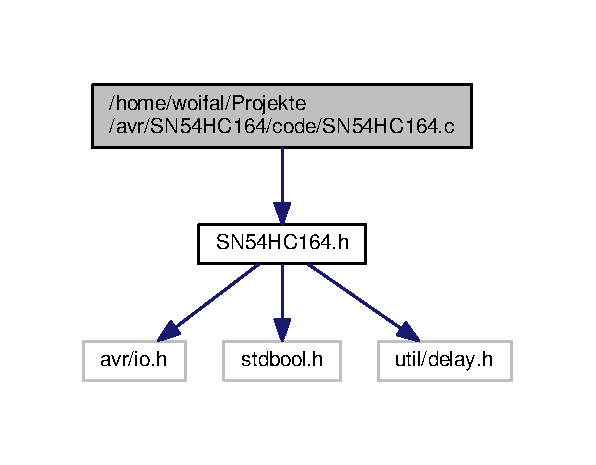
\includegraphics[width=286pt]{_s_n54_h_c164_8c__incl}
\end{center}
\end{figure}
\subsection*{Functions}
\begin{DoxyCompactItemize}
\item 
void \hyperlink{_s_n54_h_c164_8c_a3aa48ed905fd1aac09f3ca65286c354c}{S\+N54\+H\+C164\+\_\+erase} (uint8\+\_\+t $\ast$port, uint8\+\_\+t pin)
\begin{DoxyCompactList}\small\item\em Erase content of shift register. \end{DoxyCompactList}\item 
void \hyperlink{_s_n54_h_c164_8c_af3227d0693902aaba97515b8f43de590}{S\+N54\+H\+C164\+\_\+clock} (uint8\+\_\+t $\ast$data\+\_\+port, uint8\+\_\+t clock\+\_\+pin)
\begin{DoxyCompactList}\small\item\em Send clock Pulse to shift register. \end{DoxyCompactList}\item 
void \hyperlink{_s_n54_h_c164_8c_a4dad589fa4a02f265916f6744c71a970}{S\+N54\+H\+C164\+\_\+bit} (uint8\+\_\+t $\ast$data\+\_\+port, uint8\+\_\+t data\+\_\+pin, uint8\+\_\+t clock\+\_\+pin, bool bit)
\begin{DoxyCompactList}\small\item\em Shift single bit into shift register. \end{DoxyCompactList}\item 
void \hyperlink{_s_n54_h_c164_8c_a798e7d6315e25e726fa9916e6ad327dc}{S\+N54\+H\+C164\+\_\+byte} (uint8\+\_\+t $\ast$data\+\_\+port, uint8\+\_\+t data\+\_\+pin, uint8\+\_\+t clk\+\_\+pin, uint8\+\_\+t databyte)
\begin{DoxyCompactList}\small\item\em Shift whole byte into shift register. \end{DoxyCompactList}\end{DoxyCompactItemize}


\subsection{Detailed Description}
Functions for Shift Register S\+N54\+H\+C164. 

\hyperlink{_s_n54_h_c164_8c}{S\+N54\+H\+C164.\+c}

\begin{DoxyAuthor}{Author}
Woifale 
\end{DoxyAuthor}
\begin{DoxyDate}{Date}
26 July 2017 This file contains functions to work with Shift Register S\+N54\+H\+C164. S\+N54\+H\+C164 is a serial 8bit Shift register which immediately writes out data 
\end{DoxyDate}


\subsection{Function Documentation}
\hypertarget{_s_n54_h_c164_8c_a4dad589fa4a02f265916f6744c71a970}{\index{S\+N54\+H\+C164.\+c@{S\+N54\+H\+C164.\+c}!S\+N54\+H\+C164\+\_\+bit@{S\+N54\+H\+C164\+\_\+bit}}
\index{S\+N54\+H\+C164\+\_\+bit@{S\+N54\+H\+C164\+\_\+bit}!S\+N54\+H\+C164.\+c@{S\+N54\+H\+C164.\+c}}
\subsubsection[{S\+N54\+H\+C164\+\_\+bit}]{\setlength{\rightskip}{0pt plus 5cm}void S\+N54\+H\+C164\+\_\+bit (
\begin{DoxyParamCaption}
\item[{uint8\+\_\+t $\ast$}]{data\+\_\+port, }
\item[{uint8\+\_\+t}]{data\+\_\+pin, }
\item[{uint8\+\_\+t}]{clock\+\_\+pin, }
\item[{bool}]{bit}
\end{DoxyParamCaption}
)}}\label{_s_n54_h_c164_8c_a4dad589fa4a02f265916f6744c71a970}


Shift single bit into shift register. 


\begin{DoxyParams}[1]{Parameters}
\mbox{\tt in}  & {\em $\ast$data\+\_\+port} & $\ast$port is the reference -\/ an 8 bit address -\/ to the data port of the micro controller where the data port of the shift register is connected to. Please make sure to use an leading \& in case of handing over a macro definition like P\+O\+R\+T\+D. \\
\hline
\mbox{\tt in}  & {\em data\+\_\+pin} & the number of the microcontroller's pin of port handed over above (eg. P\+D3) where the data line of the shift register is connected to the micro controller. \\
\hline
\mbox{\tt in}  & {\em clock\+\_\+pin} & the number of the microcontroller's pin of port handed over above (eg. P\+D3) where the clock line of the shift register is connected to the micro controller. \\
\hline
\mbox{\tt in}  & {\em bit} & is an boolean set to either true or false. Whereby true represents 1 and false 0.\\
\hline
\end{DoxyParams}
The function set the line given by combination of data\+\_\+port and data\+\_\+pin to value according to parameter bit (true or false -\/ whereby true = high and false = low). This level is held for the periode specified in macro S\+N54\+H\+C164\+\_\+\+C\+M\+D\+\_\+\+W\+A\+I\+T\+\_\+\+D\+A\+T\+A\+\_\+\+T\+I\+M\+E. Default value is set to minimum time according spec.

After setting the data line the function  S\+N54\+H\+C164\+\_\+clock is called to instruct the shift register to take over the state given on data line.

This function requires the include $<$util/delay.\+h$>$

Usage\+: 
\begin{DoxyCode}
1 #include <avr/io.h>
2 #include <util/delay.h>
3 
4 #define SHIFT\_REG\_DATA\_PORT PORTD
5 #define SHIFT\_REG\_CLK\_PIN   PD3
6 #define SHIFT\_REG\_DATA\_PIN  PD2
7 #define SN54HC164\_CMD\_WAIT\_CLK\_TIME 25
8 #define SN54HC164\_CMD\_WAIT\_DATA\_TIME 30
9 ...
10 SN54HC164\_bit(&SHIFT\_REG\_DATA\_PORT, SHIFT\_REG\_DATA\_PIN,SHIFT\_REG\_CLK\_PIN, true);
11 ...
\end{DoxyCode}
 \hypertarget{_s_n54_h_c164_8c_a798e7d6315e25e726fa9916e6ad327dc}{\index{S\+N54\+H\+C164.\+c@{S\+N54\+H\+C164.\+c}!S\+N54\+H\+C164\+\_\+byte@{S\+N54\+H\+C164\+\_\+byte}}
\index{S\+N54\+H\+C164\+\_\+byte@{S\+N54\+H\+C164\+\_\+byte}!S\+N54\+H\+C164.\+c@{S\+N54\+H\+C164.\+c}}
\subsubsection[{S\+N54\+H\+C164\+\_\+byte}]{\setlength{\rightskip}{0pt plus 5cm}void S\+N54\+H\+C164\+\_\+byte (
\begin{DoxyParamCaption}
\item[{uint8\+\_\+t $\ast$}]{data\+\_\+port, }
\item[{uint8\+\_\+t}]{data\+\_\+pin, }
\item[{uint8\+\_\+t}]{clock\+\_\+pin, }
\item[{uint8\+\_\+t}]{databyte}
\end{DoxyParamCaption}
)}}\label{_s_n54_h_c164_8c_a798e7d6315e25e726fa9916e6ad327dc}


Shift whole byte into shift register. 


\begin{DoxyParams}[1]{Parameters}
\mbox{\tt in}  & {\em $\ast$data\+\_\+port} & $\ast$port is the reference -\/ an 8 bit address -\/ to the data port of the micro controller where the data port of the shift register is connected to. Please make sure to use an leading \& in case of handing over a macro definition like P\+O\+R\+T\+D. \\
\hline
\mbox{\tt in}  & {\em data\+\_\+pin} & the number of the microcontroller's pin of port handed over above (eg. P\+D3) where the data line of the shift register is connected to the micro controller. \\
\hline
\mbox{\tt in}  & {\em clock\+\_\+pin} & the number of the microcontroller's pin of port handed over above (eg. P\+D3) where the clock line of the shift register is connected to the micro controller. \\
\hline
\mbox{\tt in}  & {\em databyte} & a byte of data which will be shifted into the register.\\
\hline
\end{DoxyParams}
The function set the line given by combination of data\+\_\+port and data\+\_\+pin to value according to parameter databyte. Therfore the function S\+N54\+H\+C164\+\_\+bit is called for each bit of databyte.

This function requires the include $<$util/delay.\+h$>$

Usage\+: 
\begin{DoxyCode}
1 #include <avr/io.h>
2 #include <util/delay.h>
3 
4 #define SHIFT\_REG\_DATA\_PORT PORTD
5 #define SHIFT\_REG\_CLK\_PIN   PD3
6 #define SHIFT\_REG\_DATA\_PIN  PD2
7 #define SN54HC164\_CMD\_WAIT\_CLK\_TIME 25
8 #define SN54HC164\_CMD\_WAIT\_DATA\_TIME 30
9 ...
10 SN54HC164\_byte(&SHIFT\_REG\_DATA\_PORT, SHIFT\_REG\_DATA\_PIN, SHIFT\_REG\_CLK\_PIN, 0b10101010);
11 ...
\end{DoxyCode}
 \hypertarget{_s_n54_h_c164_8c_af3227d0693902aaba97515b8f43de590}{\index{S\+N54\+H\+C164.\+c@{S\+N54\+H\+C164.\+c}!S\+N54\+H\+C164\+\_\+clock@{S\+N54\+H\+C164\+\_\+clock}}
\index{S\+N54\+H\+C164\+\_\+clock@{S\+N54\+H\+C164\+\_\+clock}!S\+N54\+H\+C164.\+c@{S\+N54\+H\+C164.\+c}}
\subsubsection[{S\+N54\+H\+C164\+\_\+clock}]{\setlength{\rightskip}{0pt plus 5cm}void S\+N54\+H\+C164\+\_\+clock (
\begin{DoxyParamCaption}
\item[{uint8\+\_\+t $\ast$}]{data\+\_\+port, }
\item[{uint8\+\_\+t}]{clock\+\_\+pin}
\end{DoxyParamCaption}
)}}\label{_s_n54_h_c164_8c_af3227d0693902aaba97515b8f43de590}


Send clock Pulse to shift register. 


\begin{DoxyParams}[1]{Parameters}
\mbox{\tt in}  & {\em $\ast$data\+\_\+port} & $\ast$port is the reference -\/ an 8 bit address -\/ to the data port of the micro controller where the data port of the shift register is connected to. Please make sure to use an leading \& in case of handing over a macro definition like P\+O\+R\+T\+D. \\
\hline
\mbox{\tt in}  & {\em clock\+\_\+pin} & the number of the microcontroller's pin of port handed over above (eg. P\+D4) where the clock line of the shift register is connected to the micro controller.\\
\hline
\end{DoxyParams}
The function set the line given by combination of data\+\_\+port and clock\+\_\+pin to high. This level is held for the periode specified in macro S\+N54\+H\+C164\+\_\+\+C\+M\+D\+\_\+\+W\+A\+I\+T\+\_\+\+C\+L\+K\+\_\+\+T\+I\+M\+E. Default value is set to minimum time according spec.

This function requires the include $<$util/delay.\+h$>$

Usage\+: 
\begin{DoxyCode}
1 #include <avr/io.h>
2 #include <util/delay.h>
3 
4 #define SHIFT\_REG\_DATA\_PORT PORTD
5 #define SHIFT\_REG\_CLK\_PIN   PD4
6 #define SN54HC164\_CMD\_WAIT\_CLK\_TIME 25
7 ...
8 SN54HC164\_clock(&SHIFT\_REG\_DATA\_PORT, SHIFT\_REG\_CLK\_PIN);
9 ...
\end{DoxyCode}
 \hypertarget{_s_n54_h_c164_8c_a3aa48ed905fd1aac09f3ca65286c354c}{\index{S\+N54\+H\+C164.\+c@{S\+N54\+H\+C164.\+c}!S\+N54\+H\+C164\+\_\+erase@{S\+N54\+H\+C164\+\_\+erase}}
\index{S\+N54\+H\+C164\+\_\+erase@{S\+N54\+H\+C164\+\_\+erase}!S\+N54\+H\+C164.\+c@{S\+N54\+H\+C164.\+c}}
\subsubsection[{S\+N54\+H\+C164\+\_\+erase}]{\setlength{\rightskip}{0pt plus 5cm}void S\+N54\+H\+C164\+\_\+erase (
\begin{DoxyParamCaption}
\item[{uint8\+\_\+t $\ast$}]{port, }
\item[{uint8\+\_\+t}]{pin}
\end{DoxyParamCaption}
)}}\label{_s_n54_h_c164_8c_a3aa48ed905fd1aac09f3ca65286c354c}


Erase content of shift register. 


\begin{DoxyParams}[1]{Parameters}
\mbox{\tt in}  & {\em $\ast$port} & is the reference -\/ an 8 bit address -\/ to the data port of the micro controller where the data port of the shift register is connected to. Please make sure to use an leading \& in case of handing over a macro definition like P\+O\+R\+T\+D.\\
\hline
\mbox{\tt in}  & {\em pin} & the number of the microcontroller's pin of port handed over above (eg. P\+D4) where the erase line of the shift register is connected to the micro controller.\\
\hline
\end{DoxyParams}
The function set the C\+L\+R line to low for the periode specified in S\+N54\+H\+C164\+\_\+\+C\+M\+D\+\_\+\+W\+A\+I\+T\+\_\+\+C\+L\+R\+\_\+\+T\+I\+M\+E. By doing this the content of the shift register is set to zeros.

This function requires the include $<$util/delay.\+h$>$

Usage\+: 
\begin{DoxyCode}
1 #include <avr/io.h>
2 #include <util/delay.h>
3 
4 #define SHIFT\_REG\_DATA\_PORT PORTD
5 #define SHIFT\_REG\_CLR\_PIN   PD3
6 #define SN54HC164\_CMD\_WAIT\_CLR\_TIME 30
7 ...
8 SN54HC164\_erase(&SHIFT\_REG\_DATA\_PORT, SHIFT\_REG\_CLR\_PIN);
9 ...
\end{DoxyCode}
 
\hypertarget{_s_n54_h_c164_8h}{\section{/home/woifal/\+Projekte/avr/\+S\+N54\+H\+C164/code/\+S\+N54\+H\+C164.h File Reference}
\label{_s_n54_h_c164_8h}\index{/home/woifal/\+Projekte/avr/\+S\+N54\+H\+C164/code/\+S\+N54\+H\+C164.\+h@{/home/woifal/\+Projekte/avr/\+S\+N54\+H\+C164/code/\+S\+N54\+H\+C164.\+h}}
}


Functions for Shift Register S\+N54\+H\+C164.  


{\ttfamily \#include $<$avr/io.\+h$>$}\\*
{\ttfamily \#include $<$stdbool.\+h$>$}\\*
{\ttfamily \#include $<$util/delay.\+h$>$}\\*
Include dependency graph for S\+N54\+H\+C164.\+h\+:\nopagebreak
\begin{figure}[H]
\begin{center}
\leavevmode
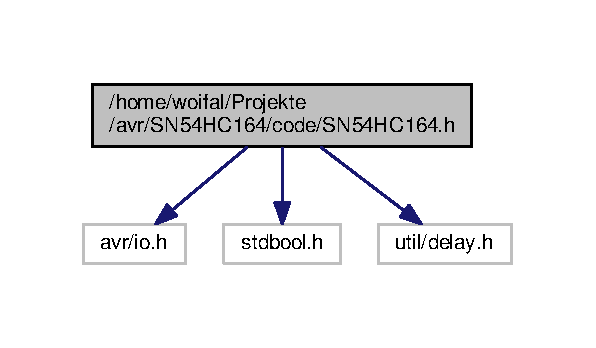
\includegraphics[width=286pt]{_s_n54_h_c164_8h__incl}
\end{center}
\end{figure}
This graph shows which files directly or indirectly include this file\+:\nopagebreak
\begin{figure}[H]
\begin{center}
\leavevmode
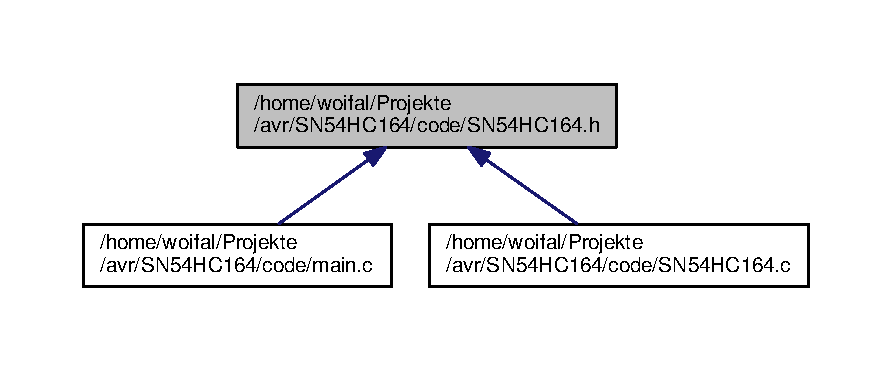
\includegraphics[width=350pt]{_s_n54_h_c164_8h__dep__incl}
\end{center}
\end{figure}
\subsection*{Macros}
\begin{DoxyCompactItemize}
\item 
\#define \hyperlink{_s_n54_h_c164_8h_a22469686577e3f812413a6eefbce7eb5}{S\+N54\+H\+C164\+\_\+\+H}
\item 
\#define \hyperlink{_s_n54_h_c164_8h_a35e9e6e2083e3b0868e9d83b2962cf88}{S\+N54\+H\+C164\+\_\+\+C\+M\+D\+\_\+\+W\+A\+I\+T\+\_\+\+C\+L\+K\+\_\+\+T\+I\+M\+E}~25
\item 
\#define \hyperlink{_s_n54_h_c164_8h_aa84d3dd4dde38f540cb59f9ec8318674}{S\+N54\+H\+C164\+\_\+\+C\+M\+D\+\_\+\+W\+A\+I\+T\+\_\+\+D\+A\+T\+A\+\_\+\+T\+I\+M\+E}~30
\item 
\#define \hyperlink{_s_n54_h_c164_8h_affcc1fc171b3c770e2de25decf2935a5}{S\+N54\+H\+C164\+\_\+\+C\+M\+D\+\_\+\+W\+A\+I\+T\+\_\+\+C\+L\+R\+\_\+\+T\+I\+M\+E}~30
\end{DoxyCompactItemize}
\subsection*{Functions}
\begin{DoxyCompactItemize}
\item 
void \hyperlink{_s_n54_h_c164_8h_a3aa48ed905fd1aac09f3ca65286c354c}{S\+N54\+H\+C164\+\_\+erase} (uint8\+\_\+t $\ast$port, uint8\+\_\+t pin)
\begin{DoxyCompactList}\small\item\em Erase content of shift register. \end{DoxyCompactList}\item 
void \hyperlink{_s_n54_h_c164_8h_af3227d0693902aaba97515b8f43de590}{S\+N54\+H\+C164\+\_\+clock} (uint8\+\_\+t $\ast$data\+\_\+port, uint8\+\_\+t clock\+\_\+pin)
\begin{DoxyCompactList}\small\item\em Send clock Pulse to shift register. \end{DoxyCompactList}\item 
void \hyperlink{_s_n54_h_c164_8h_a4dad589fa4a02f265916f6744c71a970}{S\+N54\+H\+C164\+\_\+bit} (uint8\+\_\+t $\ast$data\+\_\+port, uint8\+\_\+t data\+\_\+pin, uint8\+\_\+t clock\+\_\+pin, bool bit)
\begin{DoxyCompactList}\small\item\em Shift single bit into shift register. \end{DoxyCompactList}\item 
void \hyperlink{_s_n54_h_c164_8h_a7aed975455db966f44726caadf705ac9}{S\+N54\+H\+C164\+\_\+byte} (uint8\+\_\+t $\ast$data\+\_\+port, uint8\+\_\+t data\+\_\+pin, uint8\+\_\+t clock\+\_\+pin, uint8\+\_\+t databyte)
\begin{DoxyCompactList}\small\item\em Shift whole byte into shift register. \end{DoxyCompactList}\end{DoxyCompactItemize}


\subsection{Detailed Description}
Functions for Shift Register S\+N54\+H\+C164. 

\begin{DoxyAuthor}{Author}
Woifale 
\end{DoxyAuthor}
\begin{DoxyDate}{Date}
26 July 2017 This file contains header functions to work with Shift Register S\+N54\+H\+C164. S\+N54\+H\+C164 is a serial 8bit Shift register which immediately writes out data 
\end{DoxyDate}


\subsection{Macro Definition Documentation}
\hypertarget{_s_n54_h_c164_8h_a35e9e6e2083e3b0868e9d83b2962cf88}{\index{S\+N54\+H\+C164.\+h@{S\+N54\+H\+C164.\+h}!S\+N54\+H\+C164\+\_\+\+C\+M\+D\+\_\+\+W\+A\+I\+T\+\_\+\+C\+L\+K\+\_\+\+T\+I\+M\+E@{S\+N54\+H\+C164\+\_\+\+C\+M\+D\+\_\+\+W\+A\+I\+T\+\_\+\+C\+L\+K\+\_\+\+T\+I\+M\+E}}
\index{S\+N54\+H\+C164\+\_\+\+C\+M\+D\+\_\+\+W\+A\+I\+T\+\_\+\+C\+L\+K\+\_\+\+T\+I\+M\+E@{S\+N54\+H\+C164\+\_\+\+C\+M\+D\+\_\+\+W\+A\+I\+T\+\_\+\+C\+L\+K\+\_\+\+T\+I\+M\+E}!S\+N54\+H\+C164.\+h@{S\+N54\+H\+C164.\+h}}
\subsubsection[{S\+N54\+H\+C164\+\_\+\+C\+M\+D\+\_\+\+W\+A\+I\+T\+\_\+\+C\+L\+K\+\_\+\+T\+I\+M\+E}]{\setlength{\rightskip}{0pt plus 5cm}\#define S\+N54\+H\+C164\+\_\+\+C\+M\+D\+\_\+\+W\+A\+I\+T\+\_\+\+C\+L\+K\+\_\+\+T\+I\+M\+E~25}}\label{_s_n54_h_c164_8h_a35e9e6e2083e3b0868e9d83b2962cf88}
Wait Time in micro seconds. According to specifiction this is the minimal time the I\+C needs to recognize the Clock signal. \hypertarget{_s_n54_h_c164_8h_affcc1fc171b3c770e2de25decf2935a5}{\index{S\+N54\+H\+C164.\+h@{S\+N54\+H\+C164.\+h}!S\+N54\+H\+C164\+\_\+\+C\+M\+D\+\_\+\+W\+A\+I\+T\+\_\+\+C\+L\+R\+\_\+\+T\+I\+M\+E@{S\+N54\+H\+C164\+\_\+\+C\+M\+D\+\_\+\+W\+A\+I\+T\+\_\+\+C\+L\+R\+\_\+\+T\+I\+M\+E}}
\index{S\+N54\+H\+C164\+\_\+\+C\+M\+D\+\_\+\+W\+A\+I\+T\+\_\+\+C\+L\+R\+\_\+\+T\+I\+M\+E@{S\+N54\+H\+C164\+\_\+\+C\+M\+D\+\_\+\+W\+A\+I\+T\+\_\+\+C\+L\+R\+\_\+\+T\+I\+M\+E}!S\+N54\+H\+C164.\+h@{S\+N54\+H\+C164.\+h}}
\subsubsection[{S\+N54\+H\+C164\+\_\+\+C\+M\+D\+\_\+\+W\+A\+I\+T\+\_\+\+C\+L\+R\+\_\+\+T\+I\+M\+E}]{\setlength{\rightskip}{0pt plus 5cm}\#define S\+N54\+H\+C164\+\_\+\+C\+M\+D\+\_\+\+W\+A\+I\+T\+\_\+\+C\+L\+R\+\_\+\+T\+I\+M\+E~30}}\label{_s_n54_h_c164_8h_affcc1fc171b3c770e2de25decf2935a5}
Wait time in micro seconds. According to specification this is the minimal time the I\+C needs to recognize the clear signal. \hypertarget{_s_n54_h_c164_8h_aa84d3dd4dde38f540cb59f9ec8318674}{\index{S\+N54\+H\+C164.\+h@{S\+N54\+H\+C164.\+h}!S\+N54\+H\+C164\+\_\+\+C\+M\+D\+\_\+\+W\+A\+I\+T\+\_\+\+D\+A\+T\+A\+\_\+\+T\+I\+M\+E@{S\+N54\+H\+C164\+\_\+\+C\+M\+D\+\_\+\+W\+A\+I\+T\+\_\+\+D\+A\+T\+A\+\_\+\+T\+I\+M\+E}}
\index{S\+N54\+H\+C164\+\_\+\+C\+M\+D\+\_\+\+W\+A\+I\+T\+\_\+\+D\+A\+T\+A\+\_\+\+T\+I\+M\+E@{S\+N54\+H\+C164\+\_\+\+C\+M\+D\+\_\+\+W\+A\+I\+T\+\_\+\+D\+A\+T\+A\+\_\+\+T\+I\+M\+E}!S\+N54\+H\+C164.\+h@{S\+N54\+H\+C164.\+h}}
\subsubsection[{S\+N54\+H\+C164\+\_\+\+C\+M\+D\+\_\+\+W\+A\+I\+T\+\_\+\+D\+A\+T\+A\+\_\+\+T\+I\+M\+E}]{\setlength{\rightskip}{0pt plus 5cm}\#define S\+N54\+H\+C164\+\_\+\+C\+M\+D\+\_\+\+W\+A\+I\+T\+\_\+\+D\+A\+T\+A\+\_\+\+T\+I\+M\+E~30}}\label{_s_n54_h_c164_8h_aa84d3dd4dde38f540cb59f9ec8318674}
Wait time in micro seconds. According to specification this is the minimal time the I\+C needs to recognize data signal. \hypertarget{_s_n54_h_c164_8h_a22469686577e3f812413a6eefbce7eb5}{\index{S\+N54\+H\+C164.\+h@{S\+N54\+H\+C164.\+h}!S\+N54\+H\+C164\+\_\+\+H@{S\+N54\+H\+C164\+\_\+\+H}}
\index{S\+N54\+H\+C164\+\_\+\+H@{S\+N54\+H\+C164\+\_\+\+H}!S\+N54\+H\+C164.\+h@{S\+N54\+H\+C164.\+h}}
\subsubsection[{S\+N54\+H\+C164\+\_\+\+H}]{\setlength{\rightskip}{0pt plus 5cm}\#define S\+N54\+H\+C164\+\_\+\+H}}\label{_s_n54_h_c164_8h_a22469686577e3f812413a6eefbce7eb5}
avoids double processing of this include 

\subsection{Function Documentation}
\hypertarget{_s_n54_h_c164_8h_a4dad589fa4a02f265916f6744c71a970}{\index{S\+N54\+H\+C164.\+h@{S\+N54\+H\+C164.\+h}!S\+N54\+H\+C164\+\_\+bit@{S\+N54\+H\+C164\+\_\+bit}}
\index{S\+N54\+H\+C164\+\_\+bit@{S\+N54\+H\+C164\+\_\+bit}!S\+N54\+H\+C164.\+h@{S\+N54\+H\+C164.\+h}}
\subsubsection[{S\+N54\+H\+C164\+\_\+bit}]{\setlength{\rightskip}{0pt plus 5cm}void S\+N54\+H\+C164\+\_\+bit (
\begin{DoxyParamCaption}
\item[{uint8\+\_\+t $\ast$}]{data\+\_\+port, }
\item[{uint8\+\_\+t}]{data\+\_\+pin, }
\item[{uint8\+\_\+t}]{clock\+\_\+pin, }
\item[{bool}]{bit}
\end{DoxyParamCaption}
)}}\label{_s_n54_h_c164_8h_a4dad589fa4a02f265916f6744c71a970}


Shift single bit into shift register. 


\begin{DoxyParams}[1]{Parameters}
\mbox{\tt in}  & {\em $\ast$data\+\_\+port} & $\ast$port is the reference -\/ an 8 bit address -\/ to the data port of the micro controller where the data port of the shift register is connected to. Please make sure to use an leading \& in case of handing over a macro definition like P\+O\+R\+T\+D. \\
\hline
\mbox{\tt in}  & {\em data\+\_\+pin} & the number of the microcontroller's pin of port handed over above (eg. P\+D3) where the data line of the shift register is connected to the micro controller. \\
\hline
\mbox{\tt in}  & {\em clock\+\_\+pin} & the number of the microcontroller's pin of port handed over above (eg. P\+D3) where the clock line of the shift register is connected to the micro controller. \\
\hline
\mbox{\tt in}  & {\em bit} & is an boolean set to either true or false. Whereby true represents 1 and false 0.\\
\hline
\end{DoxyParams}
The function set the line given by combination of data\+\_\+port and data\+\_\+pin to value according to parameter bit (true or false -\/ whereby true = high and false = low). This level is held for the periode specified in macro S\+N54\+H\+C164\+\_\+\+C\+M\+D\+\_\+\+W\+A\+I\+T\+\_\+\+D\+A\+T\+A\+\_\+\+T\+I\+M\+E. Default value is set to minimum time according spec.

After setting the data line the function  S\+N54\+H\+C164\+\_\+clock is called to instruct the shift register to take over the state given on data line.

This function requires the include $<$util/delay.\+h$>$

Usage\+: 
\begin{DoxyCode}
1 #include <avr/io.h>
2 #include <util/delay.h>
3 
4 #define SHIFT\_REG\_DATA\_PORT PORTD
5 #define SHIFT\_REG\_CLK\_PIN   PD3
6 #define SHIFT\_REG\_DATA\_PIN  PD2
7 #define SN54HC164\_CMD\_WAIT\_CLK\_TIME 25
8 #define SN54HC164\_CMD\_WAIT\_DATA\_TIME 30
9 ...
10 SN54HC164\_bit(&SHIFT\_REG\_DATA\_PORT, SHIFT\_REG\_DATA\_PIN,SHIFT\_REG\_CLK\_PIN, true);
11 ...
\end{DoxyCode}
 \hypertarget{_s_n54_h_c164_8h_a7aed975455db966f44726caadf705ac9}{\index{S\+N54\+H\+C164.\+h@{S\+N54\+H\+C164.\+h}!S\+N54\+H\+C164\+\_\+byte@{S\+N54\+H\+C164\+\_\+byte}}
\index{S\+N54\+H\+C164\+\_\+byte@{S\+N54\+H\+C164\+\_\+byte}!S\+N54\+H\+C164.\+h@{S\+N54\+H\+C164.\+h}}
\subsubsection[{S\+N54\+H\+C164\+\_\+byte}]{\setlength{\rightskip}{0pt plus 5cm}void S\+N54\+H\+C164\+\_\+byte (
\begin{DoxyParamCaption}
\item[{uint8\+\_\+t $\ast$}]{data\+\_\+port, }
\item[{uint8\+\_\+t}]{data\+\_\+pin, }
\item[{uint8\+\_\+t}]{clock\+\_\+pin, }
\item[{uint8\+\_\+t}]{databyte}
\end{DoxyParamCaption}
)}}\label{_s_n54_h_c164_8h_a7aed975455db966f44726caadf705ac9}


Shift whole byte into shift register. 


\begin{DoxyParams}[1]{Parameters}
\mbox{\tt in}  & {\em $\ast$data\+\_\+port} & $\ast$port is the reference -\/ an 8 bit address -\/ to the data port of the micro controller where the data port of the shift register is connected to. Please make sure to use an leading \& in case of handing over a macro definition like P\+O\+R\+T\+D. \\
\hline
\mbox{\tt in}  & {\em data\+\_\+pin} & the number of the microcontroller's pin of port handed over above (eg. P\+D3) where the data line of the shift register is connected to the micro controller. \\
\hline
\mbox{\tt in}  & {\em clock\+\_\+pin} & the number of the microcontroller's pin of port handed over above (eg. P\+D3) where the clock line of the shift register is connected to the micro controller. \\
\hline
\mbox{\tt in}  & {\em databyte} & a byte of data which will be shifted into the register.\\
\hline
\end{DoxyParams}
The function set the line given by combination of data\+\_\+port and data\+\_\+pin to value according to parameter databyte. Therfore the function S\+N54\+H\+C164\+\_\+bit is called for each bit of databyte.

This function requires the include $<$util/delay.\+h$>$

Usage\+: 
\begin{DoxyCode}
1 #include <avr/io.h>
2 #include <util/delay.h>
3 
4 #define SHIFT\_REG\_DATA\_PORT PORTD
5 #define SHIFT\_REG\_CLK\_PIN   PD3
6 #define SHIFT\_REG\_DATA\_PIN  PD2
7 #define SN54HC164\_CMD\_WAIT\_CLK\_TIME 25
8 #define SN54HC164\_CMD\_WAIT\_DATA\_TIME 30
9 ...
10 SN54HC164\_byte(&SHIFT\_REG\_DATA\_PORT, SHIFT\_REG\_DATA\_PIN, SHIFT\_REG\_CLK\_PIN, 0b10101010);
11 ...
\end{DoxyCode}
 \hypertarget{_s_n54_h_c164_8h_af3227d0693902aaba97515b8f43de590}{\index{S\+N54\+H\+C164.\+h@{S\+N54\+H\+C164.\+h}!S\+N54\+H\+C164\+\_\+clock@{S\+N54\+H\+C164\+\_\+clock}}
\index{S\+N54\+H\+C164\+\_\+clock@{S\+N54\+H\+C164\+\_\+clock}!S\+N54\+H\+C164.\+h@{S\+N54\+H\+C164.\+h}}
\subsubsection[{S\+N54\+H\+C164\+\_\+clock}]{\setlength{\rightskip}{0pt plus 5cm}void S\+N54\+H\+C164\+\_\+clock (
\begin{DoxyParamCaption}
\item[{uint8\+\_\+t $\ast$}]{data\+\_\+port, }
\item[{uint8\+\_\+t}]{clock\+\_\+pin}
\end{DoxyParamCaption}
)}}\label{_s_n54_h_c164_8h_af3227d0693902aaba97515b8f43de590}


Send clock Pulse to shift register. 


\begin{DoxyParams}[1]{Parameters}
\mbox{\tt in}  & {\em $\ast$data\+\_\+port} & $\ast$port is the reference -\/ an 8 bit address -\/ to the data port of the micro controller where the data port of the shift register is connected to. Please make sure to use an leading \& in case of handing over a macro definition like P\+O\+R\+T\+D. \\
\hline
\mbox{\tt in}  & {\em clock\+\_\+pin} & the number of the microcontroller's pin of port handed over above (eg. P\+D4) where the clock line of the shift register is connected to the micro controller.\\
\hline
\end{DoxyParams}
The function set the line given by combination of data\+\_\+port and clock\+\_\+pin to high. This level is held for the periode specified in macro S\+N54\+H\+C164\+\_\+\+C\+M\+D\+\_\+\+W\+A\+I\+T\+\_\+\+C\+L\+K\+\_\+\+T\+I\+M\+E. Default value is set to minimum time according spec.

This function requires the include $<$util/delay.\+h$>$

Usage\+: 
\begin{DoxyCode}
1 #include <avr/io.h>
2 #include <util/delay.h>
3 
4 #define SHIFT\_REG\_DATA\_PORT PORTD
5 #define SHIFT\_REG\_CLK\_PIN   PD4
6 #define SN54HC164\_CMD\_WAIT\_CLK\_TIME 25
7 ...
8 SN54HC164\_clock(&SHIFT\_REG\_DATA\_PORT, SHIFT\_REG\_CLK\_PIN);
9 ...
\end{DoxyCode}
 \hypertarget{_s_n54_h_c164_8h_a3aa48ed905fd1aac09f3ca65286c354c}{\index{S\+N54\+H\+C164.\+h@{S\+N54\+H\+C164.\+h}!S\+N54\+H\+C164\+\_\+erase@{S\+N54\+H\+C164\+\_\+erase}}
\index{S\+N54\+H\+C164\+\_\+erase@{S\+N54\+H\+C164\+\_\+erase}!S\+N54\+H\+C164.\+h@{S\+N54\+H\+C164.\+h}}
\subsubsection[{S\+N54\+H\+C164\+\_\+erase}]{\setlength{\rightskip}{0pt plus 5cm}void S\+N54\+H\+C164\+\_\+erase (
\begin{DoxyParamCaption}
\item[{uint8\+\_\+t $\ast$}]{port, }
\item[{uint8\+\_\+t}]{pin}
\end{DoxyParamCaption}
)}}\label{_s_n54_h_c164_8h_a3aa48ed905fd1aac09f3ca65286c354c}


Erase content of shift register. 


\begin{DoxyParams}[1]{Parameters}
\mbox{\tt in}  & {\em $\ast$port} & is the reference -\/ an 8 bit address -\/ to the data port of the micro controller where the data port of the shift register is connected to. Please make sure to use an leading \& in case of handing over a macro definition like P\+O\+R\+T\+D.\\
\hline
\mbox{\tt in}  & {\em pin} & the number of the microcontroller's pin of port handed over above (eg. P\+D4) where the erase line of the shift register is connected to the micro controller.\\
\hline
\end{DoxyParams}
The function set the C\+L\+R line to low for the periode specified in S\+N54\+H\+C164\+\_\+\+C\+M\+D\+\_\+\+W\+A\+I\+T\+\_\+\+C\+L\+R\+\_\+\+T\+I\+M\+E. By doing this the content of the shift register is set to zeros.

This function requires the include $<$util/delay.\+h$>$

Usage\+: 
\begin{DoxyCode}
1 #include <avr/io.h>
2 #include <util/delay.h>
3 
4 #define SHIFT\_REG\_DATA\_PORT PORTD
5 #define SHIFT\_REG\_CLR\_PIN   PD3
6 #define SN54HC164\_CMD\_WAIT\_CLR\_TIME 30
7 ...
8 SN54HC164\_erase(&SHIFT\_REG\_DATA\_PORT, SHIFT\_REG\_CLR\_PIN);
9 ...
\end{DoxyCode}
 
%--- End generated contents ---

% Index
\newpage
\phantomsection
\addcontentsline{toc}{chapter}{Index}
\printindex

\end{document}
